\chapter{Seguridad en redes}

En el presente tema, dejaremos por un momento de lado la capa de transporte para centrarnos en la seguridad en las comunicaciones, concepto esencial que iremos detallando a lo largo de las siguientes páginas.

\subsubsection{Objetivos}
\begin{itemize}
    \item Comprender la importancia de la seguridad en las comunicaciones y aprender cómo desplegar mecanismos básicos de seguridad en redes de computadores e Internet.
    \item Conocer los aspectos de seguridad en redes: confidencialidad, autentificación, no repudio, integridad y disponibilidad. 
    \item Entender los conceptos básicos de la seguridad en redes, como el uso de algoritmos de clave secreta, de clave pública, intercambio de claves\ldots
    \item Comprender qué son los certificados digitales y las autoridades de certificación, y los diferentes mecanismos que se pueden implementar con certificados. 
    \item Conocer algunos de los principales protocolos de comunicación seguros, como \acrshort{TLS} e \acrshort{IPSec}, y los mecanismos que lo utilizan. 
\end{itemize}


\section{Introducción}
Una red de comunicaciones es \textbf{segura} cuando se garantizan todos los aspectos de seguridad, por lo que no hay protocolos ni redes 100\% seguras. No obstante, el objetivo de una red debe ser cubrir todos los aspectos de seguridad posibles.
Definamos brevemente los aspectos de seguridad que vamos a estudiar, junto con los métodos que se utilizan para garantizarlos.
\begin{itemize}
    \item \textbf{Confidencialidad / privacidad:} se garantiza que, cuando transmitimos algo a un receptor determinado, tan solo dicho receptor sea capaz de ver el mensaje.\\
    Se consigue con el cifrado. 
    \item \textbf{Autenticación:} las entidades son quien dicen ser.\\
    Se consigue con algoritmos de Reto-Respuesta o doble cifrado. 
    \item \textbf{No repudio o irrenunciabilidad:} 
    no se permite la renuncia de la autoría de determinada acción, por lo que se convierte en una prueba legal en ante un juez en el caso de ser necesario. Por ejemplo, no podemos renunciar haber participado en una transacción.\\
    Se consigue con la firma digital o con el doble cifrado con certificado, pero ha de haber una entidad fiable. 
    \item \textbf{Integridad:} se garantiza que los datos no sean manipulados por el camino (intencionadamente o no).\\
    Se consigue con funciones hash o compendios (resúmenes).
    \item \textbf{Disponibilidad:} el sistema mantiene las prestaciones de los servicios independientemente de la demanda\footnote{Este aspecto no se tratará en la asignatura.}.
\end{itemize}

Como hemos mencionado antes, una red es \textbf{segura} cuando se garantizan todos los aspectos de seguridad, y esta debe estar presente en todos los niveles de la red. El grado de seguridad lo \emph{fija el punto más débil}, ya que este es el punto más vulnerable y por el que se podría producir un ataque de seguridad. Por tanto, es importante que haya seguridad en todos los niveles de la red.

\begin{definicion}[Ataque de seguridad]
    Cualquier acción intencionada o no que menoscaba cualquiera de los aspectos de seguridad. 
\end{definicion}

Veamos algunos ejemplos de ataque de seguridad:
\begin{itemize}
    \item \textbf{Sniffing:} escuchar comunicaciones, por ejemplo mediante Wireshark. Se produce una vulneración de la confidencialidad.
    \item \textbf{Snooping (phishing):} suplantación de la identidad de alguna entidad. Se vulnera la autentificación.
    \item \textbf{Man in the Middle:} un atacante se situa en medio de dos equipos que se comunican e intercepta todos los mensajes que se transmiten.
    \item \textbf{\acrfull{DDoS}:} ataque consistente en enviar muchas peticiones a un servidor para que este no pueda atender a todas, consiguiendo que el servicio deje de funcionar. Se denomina \emph{distributed} si las peticiones provienen de distintos equipos, que suele ser lo más común. 
    \item \textbf{Malware:} software malicioso, como troyanos, gusanos, \textit{spyware}, \textit{backdoors}, \textit{rootkits}, \textit{keyloggers}, etc. Un ejemplo es \textit{ransomware}, en el que se encriptan todos o parte de los datos y se pide un rescate a cambio de estos.
\end{itemize}


Los mecanismos de seguridad que vamos a estudiar, como hemos mencionado antes, son:
\begin{itemize}
    \item Para garantizar la confidencialidad:
    \begin{itemize}
        \item Cifrado (simétrico y asimétrico).
    \end{itemize}
    \item Para garantizar la autentificación:
    \begin{itemize}
        \item Autentificación con clave secreta (reto-respuesta).
        \item Intercambio de Diffie-Hellman (establecimiento de clave secreta).
        \item Firma junto con Certificado Digital.
    \end{itemize}

    \item Para garantizar la integridad:
    \begin{itemize}
        \item Funciones Hash.
    \end{itemize}

    \item Para garantizar el no repudio:
    \begin{itemize}
        \item Firma digital y Certificados digitales.
    \end{itemize}
\end{itemize}

\section{Cifrado}
Se trata de un procedimiento para garantizar la confidencialidad, y en muchos casos también la autenticación.\\


El proceso se ilustra en la Figura~\ref{fig:cifrado/descifrado}. Inicialmente, se dispone de un texto plano a transmitir (P), que buscamos que tan solo pueda ser leído por el receptor. Para ello, se emplea una función de cifrado $E_k$ que dará lugar a un texto cifrado (C), el cual se mandará a través del canal de comunicaciones (no supone un problema, ya que este texto cifrado no será entendible). Llegará al otro extremo y será descifrado con una función $D_{k'}$, obteniendo así de nuevo el texto plano (P).

Los algoritmos de cifrado y descifrado ($E_k$ y $D_{k'}$) normalmente son conocidos, pero estos dependen de claves $k$ y $k'$ que son secretas. La dificultad reside en hallar estas claves.
\begin{figure}
    \centering
    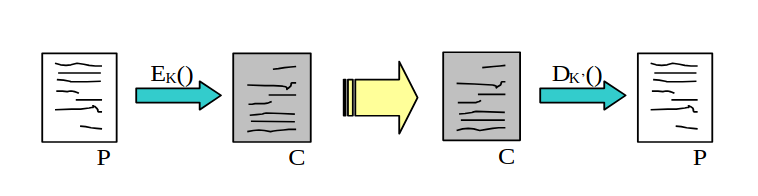
\includegraphics[width=1\linewidth]{./images/cifrado.png}
    \caption{Proceso de cifrado y descifrado.}
    \label{fig:cifrado/descifrado}
\end{figure}~\\

Veremos dos tipos de algoritmos de cifrado:
\begin{itemize}
    \item Cifrado simétrico. La clave es secreta y única ($k=k'$), y se usan distintas funciones para cifrar y descifrar.
    \item Cifrado asimétrico. Hay dos claves (pública y privada), y se usa la misma función para cifrar y descifrar.
\end{itemize}

\subsection{Cifrado simétrico}

Este tipo de algoritmos de cifrado se denomina simétrico porque se usa la misma clave para cifrar y descifrar los datos. Por tanto, la clave es secreta y tan solo es conocida por el emisor de los datos y el receptor.

\subsubsection{\acrfull{DES}}
Se trata de algoritmo de cifrado simétrico que se basa en realizar permutaciones y funciones \verb|XOR| encadenadas. Se cifran palabras de 64 bits usando una clave de 56 bits.\\

Como principal ventaja, como estas operaciones se pueden implementar de forma sencilla en hardware, es un algoritmo muy rápido, por lo que se puede usar en tiempo real (por ejemplo para codificar voz). No obstante, presenta una serie de problemas:
\begin{itemize}
    \item La longitud de la clave es corta ($2^{56}$ posibles claves), por lo que es vulnerable a ataques de fuerza bruta.
    \item Lo que se termina obteniendo es una sustitución, por lo que con la misma entrada el resultado siempre será el mismo. Usando estudios estadísticos dependiendo del idioma, se puede llegar a descifrar el mensaje.
\end{itemize}

Para mitigar este segundo aspecto, se utiliza un esquema de cifrado reentrante, donde la salida de aplicar una transformación se usa para el cifrado de la siguiente palabra a cifrar. De esta forma, quien recibe el mensaje codificado necesita conocer la última entrada usada para codificar y podrá así aplicar el proceso inverso.

\subsubsection{\acrshort{DES} doble y 3\acrshort{DES}}

Estas son distintas mejoras del algoritmo \acrshort{DES} para aumentar su seguridad y robustez. Se toman dos claves $k_1$ y $k_2$ (en el caso de 3\acrshort{DES}, podrían ser 3 distintas) y para cifrar se toma una función $E$ y su inversa $D$ y se concatenan $E_{k_1}$, $D_{k_2}$, $E_{k_1}$ y para descifrar se concatenan $D_{k_1}$, $E_{k_2}$, $D_{k_1}$.

De esta forma, podemos simular una clave de 112 bits (en el caso de 2\acrshort{DES}) o de 168 bits (en el caso de 3\acrshort{DES}); aunque se reduce la velocidad de cifrado.
\subsubsection{\acrfull{IDEA}}

Emplea la misma idea que \acrshort{DES} (cifrado empleando permutaciones y funciones \verb|XOR|), pero con claves de 128 bits en vez de 56. De esta forma, hay $2^{128}$ posibles claves, lo que reduce las posibilidades de un ataque por fuerza bruta. Los bloques que se encriptan siguen siendo de 64 bits.

\subsection{Cifrado asimétrico}
Cada usuario $A$ tiene una clave pública $K_{\text{pub}_A}$ y una clave privada $K_{\text{pri}_A}$ distintas. Conociendo la pública no es posible conocer la privada, por lo que la pública la conocen todos pero la privada solo la conoce su propietario, $A$.  Además, hay una correspondencia biunívoca entre las claves públicas y privadas.\\

Veamos ahora la forma de funcionar de estos algoritmos. Supongamos que $A$ quiere enviar un mensaje a $B$, por lo que cifraremos con la clave pública de $B$, de forma que sólo $B$ podrá descifrarlo con su clave privada. De esta forma, se garantiza la confidencialidad del mensaje. Si $P$ es el mensaje a enviar y $C$ el mensaje cifrado, se tiene que:
\begin{equation*}
    C = K_{\text{pub}_B}(P) \longrightarrow P = K_{\text{pri}_B}(C)
\end{equation*}

De cara a la autentificación, si se cifra un documento con la clave privada de $A$, se garantiza que solo $A$ ha podido cifrarlo, por lo que a priori\footnote{En el apartado dedicado a la Firga digital se verá que no es suficiente.} se garantiza la autentificación de $A$.
\begin{equation*}
    C = K_{\text{pri}_A}(P) \longrightarrow P = K_{\text{pub}_A}(C)
\end{equation*}

\subsubsection{\acrshort{RSA}}
Este algoritmo, cuyo nombre se debe a sus creadores, es ampliamente utilizado en la actualidad. Es un algoritmo de cifrado asimétrico que se basa en la factorización de números enteros.
Aunque no entraremos en el detalle de por qué es así el algoritmo\footnote{Se basa en factorización de números enteros, y se emplea para ello conocimientos mátemáticos, algunos vistos en la asignatura de Álgebra I, como la función de Euler.}, explicaremos tanto la generación de claves como el cifrado y descifrado de mensajes. Respecto a la generación de claves, se sigue el siguiente procedimiento:
\begin{enumerate}
    \item Elegimos $p,q$ primos grandes ($p,q>10^{100}$).
    \item $n = p\cdot q\qquad z = (p-1)\cdot(q-1)$.
    \item Elegimos $d$ primo relativo de $z$ ($\mcd(d,z)=1$).
    \item Calculamos $e$ tal que $e\cdot d \mod z = 1$.
\end{enumerate}
Las claves serán los siguientes pares:
\begin{equation*}
    K_{\text{pub}} = (e,n)\qquad K_{\text{pri}} = (d,n)
\end{equation*}

Para cifrar un número entero $P$ en $C$, y descifrarlo de nuevo en $P$, se usan las siguientes funciones:
\begin{align*}
    \text{Cifrado:} &\quad C = P^e \mod n\qquad \text{con } K_{\text{pub}} = (e,n)\\
    \text{Descifrado:} &\quad P = C^d \mod n \qquad \text{con } K_{\text{pri}} = (d,n)
\end{align*}

\begin{ejemplo}
    Veamos el siguiente ejemplo de aplicación del algoritmo.
    \begin{enumerate}
        \item Elegimos $p=3$ y $q=11$.
        \item $n = 3\cdot 11 = 33\qquad z = (3-1)\cdot(11-1) = 20$.
        \item Elegimos $d=7$, ya que $\mcd(7,20)=1$.
        \item Tomamos $e=3$, ya que $3\cdot 7 \mod 20 = 1$.
        \item Tenemos $K_{\text{pub}} = (3,33)$ y $K_{\text{pri}} = (7,33)$.
    \end{enumerate}

    Suponemos que queremos codificar la palabra ``SUZANNE''. Para ello, asignamos un número a cada letra (el orden en el alfabeto sin la ñ), y el proceso se ilustra en la Tabla~\ref{tab:rsa}. Notemos que, por la red, tan solo se envía el número cifrado, $C$, y no se podría descifrar sin conocer la clave privada.
    \begin{table}[H]
        \centering
        \begin{tabular}{cc||c||cc}
            Simbólico & Numérico ($P$) & $C=P^3\mod 33$ & $P=C^7\mod 33$ & Simbólico\\
            \hline
            S & 19 & 28 & 19 & S\\
            U & 21 & 21 & 21 & U\\
            Z & 26 & 10 & 26 & Z\\
            A & 1 & 1 & 1 & A\\
            N & 14 & 5 & 14 & N\\
            N & 14 & 5 & 14 & N\\
            E & 5 & 26 & 5 & E
        \end{tabular}
        \caption{Cifrado y descifrado de la palabra ``SUZANNE''.}
        \label{tab:rsa}
    \end{table}
\end{ejemplo}

\section{Autenticación}
Pongámonos en el supuesto de que dos equipos, $A$ y $B$, quieren autenticarse. Lo más sencillo es que cada uno tenga una base de datos con el usuario y la clave que comparten con el otro. Para autenticarse $A$, este le manda a $B$ su usuario y su clave compartida, y $B$ comprueba si son correctos. De forma análoga, $B$ se autentica con $A$. Al estar enviándose la clave, este método es vulnerable, pero se usa en muchos servicios, como en el protocolo \acrshort{PAP}. Se pueden hacer algunas mejoras, como enviar la información a través de túneles cifrados, pero la vulnerabilidad sigue presente.\\

Para evitar este problema, se pueden usar algoritmos de reto-respuesta.
\subsection{Reto-respuesta}
Este algoritmo se ilustra en la Figura~\ref{fig:reto-respuesta}.
Al igual que antes, supongamos que dos equipos $A$ y $B$ quieren autenticarse. Ambos tienen una base de datos que contiene, para cada usuario, la clave que comparten. Para autenticarse $A$ con $B$, este envía su identidad (usuario) $A$ (que no es un dato sensible), y $B$ le contesta con un número aleatorio $(R_B)$ denominado reto. Usando la clave compartida $K_{AB}$, $A$ cifra el reto ($K_{AB}(R_B)$) y se lo envía a $B$. El quipo $B$ también cifra el reto con la clave compartida que posee en su base de datos, y si coincide con el que ha recibido, $A$ queda autenticado. Además, $A$ habrá enviado ya un reto $R_A$ a $B$ para que este se autentique de la misma forma. De esta forma, se garantiza la autenticación de ambos equipos.\\
\begin{figure}
    \centering
    \begin{tikzpicture}[
        node distance=2cm and 1.5cm,
        every node/.style={font=\small},
        box/.style={draw, rounded corners, fill=yellow!20, minimum width=2.5cm, minimum height=0.8cm, align=center},
        entity/.style={draw, fill=green!20, minimum width=1cm, minimum height=4.5cm, align=center},
        arrow/.style={-{Latex[length=2mm, width=2mm]}}
    ]
    
    % Nodes
    \node[entity] (A) {$A$};
    
    
    \node[box, right=3cm of A.north, yshift=-0.5cm] (msg1) {$A$};
    \node[box, below=0.1cm of msg1] (msg2) {$R_B$};
    \node[box, below=0.1cm of msg2] (msg3) {$K_{AB}(R_B)$};
    \node[box, below=0.1cm of msg3] (msg4) {$R_A$};
    \node[box, below=0.1cm of msg4] (msg5) {$K_{AB}(R_A)$};

    \node[entity, right=7.5cm of A] (B) {$B$};
    
    % Arrows
    % Bucle para los que van hacia la derecha
    \foreach \i in {1,3,4}{
        \draw (msg\i.west) -- ++(-2.5cm,0);
        \draw[arrow] (msg\i.east) -- ++(2.5cm, 0);
    }

    % Bucle para los que van hacia la izquierda
    \foreach \i in {2,5}{
        \draw (msg\i.east) -- ++(2.5cm,0);
        \draw[arrow] (msg\i.west) -- ++(-2.5cm, 0);
    }

    
    \end{tikzpicture}
    \caption{Algoritmo de reto-respuesta.}
    \label{fig:reto-respuesta}
\end{figure}

Notemos que por la red no se envía ningún dado sensible, sino que solo se envían números aleatorios cifrados. Aunque parece seguro, este algoritmo tiene algunas vulnerabilidades:
\begin{itemize}
    \item \textbf{Ataque por repetición:} el atacante escucha por mucho tiempo y va guardando las respuestas correctas para cada resto. De esta forma, cuando se repita un reto, ya sabe qué respuesta ha de enviar para identificarse él, suplantando así la identidad. \textbf{Solución:} que el reto no se pueda repetir (denominado \emph{nonce}), como puede ser el instante de tiempo junto a un número aleatorio (por ejemplo).
    \item \textbf{Ataque por reflexión:} el atacante, tras escuchar el reto de $B$, le envía a $B$ su mismo reto, como si este fuese el reto de $A$. Cuando $B$ le responda, le reenvía dicha respuesta a $B$ como si hubiese sido él quien la ha cifrado. \textbf{Solución:} usar dominios de retos disjuntas, para que así no se pueda reenviar el reto de $B$ a $B$.
\end{itemize}

\subsection{Intercambio de Diffie-Hellman}

Aunque en el algoritmo de reto-respuesta no se envían claves, estas se han tenido que establecer en algún momento.
Además, también es posible que no sea posible almacenar las claves en las bases de datos mencionadas, y que tengamos que calcular una clave secreta y compartida en cada autenticación. Estos dos problemas se resuelven con el intercambio de Diffie-Hellman, ya que este algoritmo permite establecer una clave secreta entre dos entidades a través de un canal no seguro.

El algoritmo se muestra en la Figura~\ref{fig:diffie-hellman}. Aunque tampoco entraremos en detalle en las matemáticas que hay detrás, el algoritmo para crear una clave secreta compartida entre $A$ y $B$ es el siguiente:
\begin{enumerate}
    \item $A$ elige enteros $x,n$ y $g$, y $B$ elige el entero $y$.
    \item $A$ envía a $B$ los valores $g$, $n$ y $g^x \mod n$.
    \item $B$ envía a $A$ el valor $g^y \mod n$, que calcula a partir de los valores recibidos.
    \item La clave secreta que comparten $A$ y $B$, que nunca se ha transmitido por la red y, como no se ha transmitido ni $x$ ni $y$, tampoco la podrá calcular un atacante, es:
    \begin{align*}
        K_{AB}  &= (g^y \mod n)^x \mod n = g^{xy} \mod n\\
        K_{BA}  &= (g^x \mod n)^y \mod n = g^{xy} \mod n
    \end{align*}
\end{enumerate}
\begin{figure}
    \centering
    \begin{tikzpicture}[
        node distance=2cm and 1.5cm,
        every node/.style={font=\small},
        box/.style={draw, rounded corners, fill=yellow!20, minimum width=3.5cm, minimum height=0.8cm, align=center},
        entity/.style={draw, fill=green!20, minimum width=1cm, minimum height=3cm, align=center},
        arrow/.style={-{Latex[length=2mm, width=2mm]}}
    ]
    
    % Nodes
    \node[entity] (A) {$A$};
    
    
    \node[box, right=3cm of A.north, yshift=-1cm] (msg1) {$n,~g,~~~g^x\mod n$};
    \node[box, below=0.1cm of msg1] (msg2) {$g^y \mod n$};

    \node[entity, right=8.5cm of A] (B) {$B$};
    
    % Arrows
    % Bucle para los que van hacia la derecha
    \foreach \i in {1}{
        \draw (msg\i.west) -- ++(-2.5cm,0);
        \draw[arrow] (msg\i.east) -- ++(2.5cm, 0);
    }

    % Bucle para los que van hacia la izquierda
    \foreach \i in {2}{
        \draw (msg\i.east) -- ++(2.5cm,0);
        \draw[arrow] (msg\i.west) -- ++(-2.5cm, 0);
    }

    \node[above of=A,yshift=0.1cm] {$A$ elige $x,n,g$};
    \node[above of=B, yshift=0.1cm] {$B$ elige $y$};

    \node[below of=A, yshift=-0.1cm] {
        $\begin{array}{rl}
            K_{AB} & = (g^y \mod n)^x \mod n \\
                & = g^{xy} \mod n
        \end{array}$
    };
    \node[below of=B, yshift=-0.1cm] {
        $\begin{array}{rl}
            K_{BA} & = (g^x \mod n)^y \mod n \\
                & = g^{xy} \mod n
        \end{array}$
    };
    \end{tikzpicture}
    \caption{Algoritmo de intercambio de Diffie-Hellman.}
    \label{fig:diffie-hellman}
\end{figure}

No obstante, este algoritmo también tiene sus vulnerabilidades. Por ejemplo, puede sufrir un ataque del tipo \textit{man-in-the-middle}, en el que un atacante se sitúa entre $A$ y $B$ y se hace pasar por $A$ ante $B$ y por $B$ ante $A$. De esta forma, hace de mensajero invisible, y las claves compartidas en realidad serán con el atacante.

\section{Funciones Hash}

Las funciones hash son funciones de forma que, dado un texto de entrada $M$ de longitud variable, nos proporcionan un resumen (también llamado compendio) $R$ de longitud fija. Estas funciones son unidireccionales e irreversibles; es decir, a partir de un resumen $R$ no se puede obtener el mensaje original $M$. Estas deben además ser de cálculo sencillo, pues se usan en muchos protocolos de comunicación y han de poder calcularse rápidamente. Además, son invulnerables a ataques de colisión; es decir, dos mensajes distintos no pueden tener el mismo resumen.\\



Su principal utilidad es garantizar la \textbf{integridad} de un mensaje enviado. Un mensaje $M$ se enviará junto al resumen $R$ de este, y el receptor, tras recibir el mensaje, calculará el resumen del mensaje, $R'$, y comprobará si coincide con el resumen recibido. En tal caso, se garantiza que el mensaje no ha sido modificado en el camino.\\

No obstante, podría ocurrir que un atacante interceptase el mensaje y lo modificase, cambiando $M$ por $M'$ y $h(M)$ por $h(M')$. Para evitar esto, hay varias alternativas:
\begin{itemize}
    \item Cifrar el hash con la clave compartida, de forma que el atacante no podría cifrar $h(M')$ por no conocer la clave.
    \item El resumen puede incluir también a la clave compartida entre las entidades. A estos mensajes ($M$ junto a $h(K\mid B)$) se les denomina \acrfull{HMAC}.
\end{itemize}
De ambas formas, también se garantiza la autenticación del emisor del mensaje. La confidencialidad no obstante no se garantiza, pues el mensaje no se cifra, sino que se envía en texto plano.

\subsubsection{\acrfull{MD5}}

Se trata de una función hash que, dado un mensaje, nos proporciona un resumen de 128 bits. Su funcionamiento se muestra en la Figura~\ref{fig:md5}, y se desarrolla a continuación.\\

Como el algoritmo trabaja sobre bloques de 512 bits, el mensaje será \emph{siempre} extendido hasta que su longitud sea congruente con 448 módulo 512 (es decir, notando por $K$ a su longitud, se extiende hasta que $K\equiv 448\mod 512$, o lo que es lo mismo, hasta que $K-448\mod 512 = 0$). Esta extensión se hace añadiendo un $1$ seguido de ceros hasta que se cumpla la congruencia, y se hace \emph{siempre} (aunque la longitud del mensaje ya sea congruente con 448 módulo 512).

A continuación, se añade un campo de longitud de 64 bits, que indica la longitud del mensaje original. Si la longitud del mensaje original era mayor a $2^{64}$, se toman los 64 bits de menor peso.\\

Tras añadir este campo de 64 bits, como $448+64=512$, el mensaje ya tendrá longitud múltiplo de 512, por lo que se divide en bloques de 512 bits, que son a los que les aplicaremos la función hash. Se hace un procesamiento secuencial por bloques, teniendo en cuenta que la salida tras procesar un bloque sirve como entrada para procesar el siguiente. El resumen se obtendrá tras procesar el último bloque.
\begin{figure}
    \centering
    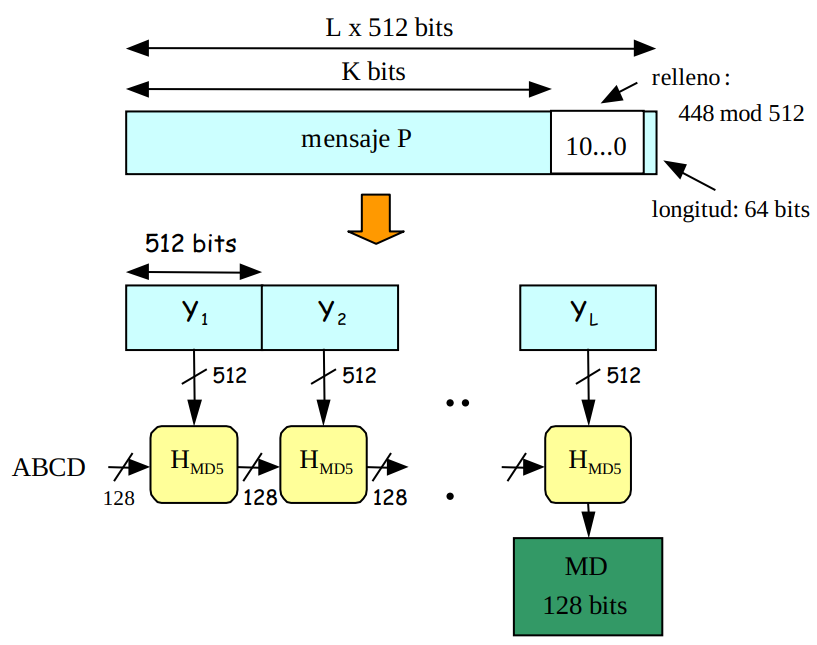
\includegraphics[width=0.7\linewidth]{./images/hash.png}
    \caption{Funcionamiento de la función hash \acrshort{MD5}.}
    \label{fig:md5}
\end{figure}

\subsubsection{\acrfull{SHA-1}}

El funcionamiento, desde el punto de vista de usuario\footnote{No entraremos en detalle en cómo está implementada como tal la función hash, aunque evidentemente son distintas.}, es análogo al de \acrshort{MD5}, ya que también se procesan bloques de 512 bits; aunque en este caso los resúmenes son de 160 bits.

\subsection{Ataque por Extensión}

Supongamos que una entidad $A$ quiere enviarle un mensaje $M$ a otra entidad $B$. Para garantizar la integridad del mensaje, lo enviará junto a su resumen, y para evitar que estos sean reemplazados por un atacante, el resumen también se hará de la clave compartida; es decir, se enviará $M$ junto a $h(K_{AB}\mid M)$.\\

Supongamos no obstante que hay un atacante escuchando, y que intercepta el mensaje $M$ junto al resumen calculado. Aunque no puede cambiar completamente $M$, sí podrá añadirle información (de ahí el nombre de extensión). Con el mensaje $M$, puede rellenarlo tal y como se describe en las funciones anteriores, y después de convertirlo a un mensaje con longitud múltiplo de 512, puede añadir al mensaje lo que quiera, obteniendo así un mensaje modificado $M'$. Para calcular $h(K_{AB}\mid M')$, como desconoce la clave compartida, no podrá hacerlo de forma directa. No obstante, como hemos visto que las funciones hash se basan en realimentación, podría usar el resumen $h(K_{AB}\mid M)$ que ha interceptado como entrada para el primer bloque que él haya añadida. De esta forma, cuando el mensaje llegue a $B$, este calculará el resumen de $M'$, que coincidirá con el que ha calculado el atacante, creyendo por tanto que el mensaje no ha sido modificado y produciéndose una vulnerabilidad.\\

Para evitar este problema, el \acrshort{HMAC} que en realidad se envía es:
\begin{equation*}
    h\left(K_{AB}\mid h(K_{AB}\mid M)\right)
\end{equation*}
De esta forma, el atacante podrá modificar el resumen calculado en la función exterior, pero nunca podrá calcular ni modificar el resumen que hay en el interior, ya que no conoce la clave compartida.

\section{Firma digital y certificados digitales}

Una \textbf{firma digital} intenta ser un sustituto de una firma escrita para poder garantizar el \textbf{no repudio} en nuestras acciones en Internet. Con ellas conseguimos:
\begin{itemize}
    \item Autenticación del firmante frente al receptor.
    \item No repudio por parte del firmante.
    \item El firmante obtiene garantía de no falsificación, proporcionando integridad.
    \item Se garantiza la confidencialidad del mensaje entre el firmante y el receptor.
\end{itemize}

Hay dos tipos de firmas digitales, mediante clave secreta o mediante doble cifrado.
\subsection{Firma digital con clave secreta. \emph{Big Brother}.}

Este método se basa el uso de una entidad fiable, denominada \emph{Big Brother} o \emph{BB}, en la que todos los usuarios confían (posiblemente sea del estado). Este comparte una clave con cada una de las entidades, de forma que todos los mensajes pasan por él. De esta forma, si surge algún problema, el Big Brother puede demostrar ante un juez quién ha hecho una transacción, en qué momento, etc.

Supongamos que $A$ quiere enviarle un mensaje $P$ a $B$ firmado digitalmente. La forma de hacerlo se ilustra en la Figura~\ref{fig:big-brother}. En primer lugar, $A$ le envía al Big Brother un mensaje que contiene:
\begin{itemize}
    \item {$A$}: Identificador de $A$.
    \item {$B$}: Identificador de $B$, el destinatario.
    \item {$R_A$}: Resumen del mensaje para garantizar la integridad.
    \item {$t$}: Instante de tiempo.
    \item {$P$}: Mensaje a enviar, en texto plano.
\end{itemize}
Notemos que, exceptuando el identificador de $A$, el resto de campos van cifrados con la clave que comparte $A$ con el Big Brother, proporcinando así confidencialidad con el BB y atenticándose así $A$. El mensaje es recibido por el BB, que lo descifra, identificando así que tiene que reenviarlo a $B$. Para ello, añade:
\begin{itemize}
    \item {$K_{BB}(A,t,P)$}: Datos de la transacción, cifrados con la clave del BB, que solo él posee y por tanto se convierte en una prueba ante un juez. Se consigue así el no repudio.
\end{itemize}
Todo esto va cifrado con la clave que comparte $B$ con el BB, garantizando así la confidencialidad del mensaje.
\begin{figure}
    \centering
    \begin{tikzpicture}[
        node distance=2cm and 1.5cm,
        every node/.style={font=\small},
        box/.style={draw, rounded corners, fill=yellow!20, minimum width=5.5cm, minimum height=0.8cm, align=center},
        entity/.style={draw, fill=green!20, minimum width=1cm, minimum height=3cm, align=center},
        arrow/.style={-{Latex[length=2mm, width=2mm]}}
    ]
    
    % Nodes
    \node[entity] (A) {$A$};
    \node[entity, right=6.6cm of A] (BB) {$BB$};
    \node[entity, right=6.6cm of BB] (B) {$B$};
    
    \node[box, right=1.05cm of A.north, yshift=-1cm] (msg1) {$A,K_A(B,R_A,t,P)$};
    \node[box, right=1.05cm of BB.north, yshift=-2cm] (msg2) {$K_B(A,R_A,t,P,K_{BB}(A,t,P))$};

    
    % Arrows
    % Bucle para los que van hacia la derecha
    \foreach \i in {1,2}{
        \draw (msg\i.west) -- ++(-0.55cm,0);
        \draw[arrow] (msg\i.east) -- ++(0.55cm, 0);
    }
    \end{tikzpicture}
    \caption{Firma digital con clave secreta. \emph{Big Brother}.}
    \label{fig:big-brother}
\end{figure}


\subsection{Firma digital con clave asimétrica. Doble cifrado}

Supongamos que $A$ le quiere mandar un mensaje a $B$. La idea se basa en lo siguiente:
\begin{itemize}
    \item Cifrar con $K_{\text{pri}_A}$ garantiza autenticación, ya que solo $A$ ha podido cifrarlo.
    \item Cifrar con $K_{\text{pub}_B}$ garantiza confidencialidad, ya que solo $B$ podrá descifrarlo.
\end{itemize}
De esta manera, realizando ambos cifrados se garantiza la autenticación y la confidencialidad del mensaje. El orden de los cifrados no importa, pero ha de establecerse previamente para que el destinatario sepa cómo descifrarlo.
\begin{align*}
    C&=K_{\text{pub}_B}\left(K_{\text{pri}_A}(P)\right)\\
    P&=K_{\text{pub}_A}\left(K_{\text{pri}_B}(C)\right)
\end{align*}

Sin embargo todo esto no garantiza el \textbf{no repudio}, puesto que nada nos garantiza que $K_{\text{pri}_A}$ sea realmente de $A$. Para garantizarlo, necesitamos los \textbf{certificados digitales}, que son emitidos por autoridades de certificación.


\subsubsection{Certificado digital}

\begin{definicion}[Autoridades de certificación]
    Entidad fiable (posiblemente del estado) que garantiza la asociación entre identidad y claves. En España, por ejemplo, la más extendida es la \acrshort{FNMT}, aunque hay otras.
\end{definicion}

En primer lugar, el usuario obtiene sus claves pública y privada y envía una solicitud firmada digitalmente a la Autoridad de Certificación. Esta, tras comprobar la firma y que el solicitante es quien dice ser, emite el certificado digital solicitado, que contiene (entre otros campos):
\begin{itemize}
    \item Identidad de la Autoridad de Certificación.
    \item Identidad del usuario.
    \item Clave pública del usuario.
\end{itemize}
Cualquier persona puede consultar este certificado digital, comprobando así que la clave pública que se le proporciona es realmente de la persona que dice ser. Para evitar falsificaciones, el certificado se cifra con la $K_{\text{priv}_\text{AC}}$ de la Autoridad de Certificación, de forma que solo esta ha podido ser la emisora del certificado.\\

El formato de certificados digitales más extendido es el estándar X.509, cuyos campos son:
\begin{itemize}
    \item Versión del estándar X.509.
    \item Número de serie único, usado por la Autoridad de Certificación para identificar el certificado.
    \item Algoritmo empleado para calcular las claves.
    \item Identidad de la Autoridad de Certificación que ha emitido el certificado.
    \item Periodo de validez del certificado.
    \item Usuario al que se le ha emitido el certificado.
    \item Clave pública del usuario al que se le ha emitido el certificado.
\end{itemize}

\section{Protocolos seguros}
La seguridad se divide en dos tipos:
\begin{itemize}
    \item \textbf{Perimetral:} consiste en garantizar la seguridad dentro de una misma red. Se usan firewalls, \acrfull{IDS} o \acrfull{IRS}.
    
    \item \textbf{Seguridad en protocolos:} si no podemos garantizar la seguridad en la red (o aun así, queremos mejorar la seguridad), se usan protocolos seguros para garantizar seguridad. Como vimos, estos han de establecerse en todas las capas, pues la seguridad la fija el punto más débil.
    \begin{itemize}
        \item Capa de aplicación: \acrshort{PGP} o \acrshort{SSH}.
        \item Capa de sesión\footnote{Entre aplicación y transporte. Ver Tabla~\ref{tab:mod_osi} correspondiente al Modelo \acrshort{OSI}.}: \acrshort{TLS} o \acrshort{SSL}.
        \item Capa de red: \acrshort{IPSec}.
    \end{itemize}
\end{itemize}

\subsection{Seguridad en la Capa de Aplicación. \acrshort{PGP}.}

En capa de aplicación deben usarse protocolos distintos para garantizar la seguridad en cada uno de los servicios prestados. Uno de ellos, el protocolo \acrfull{PGP}, tiene como objetivo garantizar la seguridad en el correo electrónico.\\

Supongamos que $A$ quiere enviar un mensaje $P$ a $B$ mediante el correo electrónico. El protocolo se ilustra en la Figura~\ref{fig:pgp}.
Al enviar $A$ el correo, el proceso es el siguiente:
\begin{enumerate}
    \item Se hace un resumen del mensaje mediante el algoritmo \acrshort{MD5}, $R=\text{MD5}(P)$.
    \item Este se firma digitalmente con la clave privada de $A$, $FD=K_{\text{pri}_A}(R)$.
    \item Tanto el mensaje como resumen cifrado se comprimen (para enviar menos datos) usando para ello el el formato ZIP\@, $Z=\text{ZIP}(FD+P)$.
    \item Se genera una clave privada específica para ese mensaje, $K$, y se cifra $Z$ con esta clave usando para ello el algoritmo de \acrshort{IDEA}, $\text{IDEA}_K(Z)$.  A esta clave $K$ se le denomina \emph{clave de sesión}, pues solo se usa en esa sesión. Notemos que, si un atacante la consigue, tan solo podrá descifrar ese mensaje, y no otros.
    \item Se cifra también la clave de sesión con la clave pública de $B$, $K_{\text{pub}_B}(K)$, para que solo $B$ pueda obtener dicha clave y, por tanto, descifrar el mensaje. Por tanto, el mensaje cifrado es $C=K_{\text{pub}_B}(K)+\text{IDEA}_K(Z)$.
    \item Este mensaje cifrado se codifica con el sistema Base64\footnote{No tiene que ver con seguridad y no se verá en la asignatura. Es una forma de codificar mensajes para enviar por internet.}, $M=\text{Base64}(C)$,
    y será el que se envíe por internet.
\end{enumerate}
\begin{figure}
    \centering
    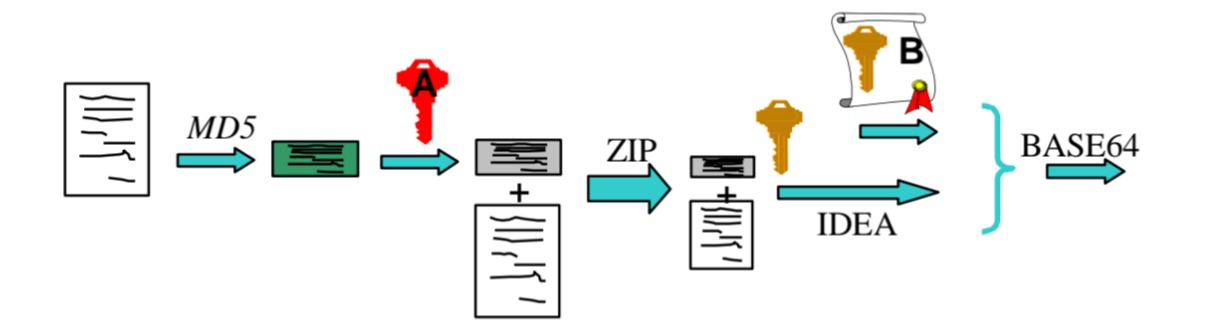
\includegraphics[width=0.8\textwidth]{images/pgp.jpeg}
    \caption{Protocolo \acrshort{PGP}.}
    \label{fig:pgp}
\end{figure}

El receptor, por su parte, cuando reciba el mensaje $M$, hará el proceso inverso:
\begin{enumerate}
    \item Decodificará el mensaje usando Base64, $C=\text{Base64}^{-1}(M)=K_{\text{pub}_B}(K)+\text{IDEA}_K(Z)$.
    \item Descifrará la clave de sesión con su clave privada, $K=K_{\text{pri}_B}\left(K_{\text{pub}_B}(K)\right)$.
    \item Descifrará el mensaje con la clave de sesión, $Z=\text{IDEA}^{-1}_K\left(\text{IDEA}_K(Z)\right)$.
    \item Descomprimirá el mensaje, $FD+P=\text{ZIP}^{-1}(Z)$.
    \item Se obtiene el resumen recibido, $R=K_{\text{pub}_A}(FD)$.
    \item Se calcula el resumen del mensaje recibido, $R'=\text{MD5}(P)$.
    \item Para comprobar que no se ha modificado, se comprueba si el resumen calculado es el mismo que el recibido, $R=R'$.
\end{enumerate}

En resumen, tenemos lo siguiente:
\begin{equation*}
    \begin{array}{l}
        \qquad \text{\ul{Emisor}}\ (A)\\\\
        R = \text{MD5}(P)\\
        FD = K_{\text{pri}_A}(R)\\
        Z = \text{ZIP}(FD+P)\\
        \text{Generación}\ K \\
        C = K_{\text{pub}_B}(K)+\text{IDEA}_K(Z)\\
        M = \text{Base64}(C)
    \end{array}
    \hspace{2cm}
    \begin{array}{l}
        \qquad \text{\ul{Receptor}}\ (B)\\\\
        C = \text{Base64}^{-1}(M)\\
        K = K_{\text{pri}_B}\left(K_{\text{pub}_B}(K)\right)\\
        Z = \text{IDEA}^{-1}_K\left(\text{IDEA}_K(Z)\right)\\
        FD+P = \text{ZIP}^{-1}(Z)\\
        R = K_{\text{pub}_A}(FD)\\
        R' = \text{MD5}(P)\\
        \text{¿}\ R = R'\ \text{?}
    \end{array}
\end{equation*}

Con este proceso conseguimos garantizar los siguientes aspectos de seguridad:
\begin{itemize}
    \item Confidencialidad: el mensaje va cifrado con la clave pública de $B$, luego solo $B$ podrá descifrarlo.
    \item Integridad: gracias al resumen, comprobamos que el mensaje no se ha modificado.
    \item Autenticación: gracias al cifrado con la clave privada de $A$, $B$ sabe que el mensaje viene de $A$.
    \item No repudio: Tan solo si hay un certificado digital de $A$ emitido por una Autoridad de Certificación, $B$ podrá demostrar que el mensaje viene de $A$.
\end{itemize}


\subsection{Seguridad en la Capa de Sesión. \acrshort{SSL} y \acrshort{TLS}.}

Esta capa ofrece servicios de seguridad empleados por gran variedad de protocolos de aplicación, como \acrshort{HTTPS}, \acrshort{IMAPS}, \acrshort{SSL}-\acrshort{POP} o \acrshort{VPN}. Los principales protocolos de esta capa son \acrshort{SSL} y \acrshort{TLS}, que en esencia crean túneles cifrados para el intercambio de información.

\subsubsection{\acrfull{SSL}}
En realidad, no es un protocolo sino una familia de ellos que se usan de forma conjunta.
\begin{itemize}
    \item \ul{\acrshort{SSL} Handshake Protocol}: se negocia el algoritmo de cifrado y la función hash; y el servidor se autentica con un certificado digital del tipo {X.509}. El cliente genera claves de sesión (de esta forma, si un atacante la consigue tan solo podrá obtener los mensajes de esa sesión), y hay dos opciones para ello:
    \begin{itemize}
        \item Se generan aleatoriamente y se envían cifradas con la clave pública del servidor (este ya se ha autenticado).
        \item Se generan mediante el intercambio de Diffie-Hellman. El problema del ``man-in-the-middle'' no se tiene en este caso, pues el servidor ya se ha autenticado.
    \end{itemize}

    \item \ul{\acrshort{SSL} Assert Protocol}: informa sobre errores en la sesión.
    \item \ul{Change Cipher Spec Protocol}: usado para notificar cambios en el cifrado.

    \item \ul{\acrshort{SSL} Record Protocol}: encapsula los protocolos anteriores, y ofrece un canal seguro.\\
    
    Para enviar datos, se hace lo siguiente:
    \begin{enumerate}
        \item Se fragmenta el mensaje en fragmentos denominados \emph{registros}.
        \item Cada registro es comprimido, y al comprimido se le calcula un resumen mediante la función hash acordada.
        \item Se cifra el mensaje comprimido junto con su resumen mediante la clave de sesión.
        \item Esto será lo que trasmite, encapsulado en un paquete \acrshort{TCP}.
    \end{enumerate}
    
    Se garantiza \emph{confidencialidad} (pues se cifra), \emph{integridad} (pues se calcula el resumen) y \emph{autenticación} por parte del servidor (pues se ha autenticado con su firma y certificado digital).
\end{itemize}



\subsubsection{TLS}

\subsection{IPSec}
Su objetivo es garantizar autenticación, integridad y opcionalmente privacidad a nivel IP\@. Crea túneles unidireccionales. 

\begin{definicion}[Túnel]
    Es un sitio donde entra un paquete y a la salida tendremos exactamente el mismo paquete. Para ello encapsulamos el paquete dentro de otro paquete. Si el túnel va cifrado (la parte de los datos va cifrada) entonces el túnel es seguro.
\end{definicion}

Son tres procedimientos:
\begin{enumerate}
    \item Establecimiento de una ``Asociación de seguridad'': con el objetivo de establecer una clave secreta (Diffie-Hellman), con la previa autenticación. Es simplex. Vulnera el carácter NO orientado a conexión. 
    \item Garantizar la autenticación e integridad de los datos mediante las ``Cabeceras de autenticación''.
    \item (Opcional) Garantizar la privacidad de los datos mediante el protocolo de ``Encapsulado de seguridad de la carga''.
\end{enumerate}

Dos tipos de túneles:
\begin{itemize}
    \item Modo transporte: la asociación se hace extremo a extremo entre el host origen y destino.
    \item Modo túnel: la asociación se hace entre dos routers intermediarios. Útil por ejemplo si una empresa quiere comunicar dos sucursales, en vez de comunicar cada dos trabajadores, se comunican mediante esos routers intermediarios y solo hacen falta dos túneles (para ambas direcciones).
\end{itemize}


